%\documentclass[aip,pop,amsmath,amssymb]{revtex4-1}
\documentclass[aip,reprint]{revtex4-1}

\draft 

\usepackage{graphicx}
\usepackage{dcolumn}
\usepackage{bm}
\usepackage{braket}
\usepackage{amsmath}
\usepackage{hyperref}
\usepackage{amssymb}
\usepackage{hhline}
\usepackage{xfrac}
\usepackage{color}   %May be necessary if you want to color links

\hypersetup{
    colorlinks=true, %set true if you want colored links
    linkcolor=blue,  %choose some color if you want links to stand out
    citecolor=blue,
    urlcolor=blue
}

\newcommand{\ignore}[2]{\hspace{0in}#2}
\newcommand{\Lagr}{\mathcal{L}}
\newcommand{\Recy}{\mathcal{R}}
\newcommand{\Eps}{\mathcal{E}}
\newcommand{\ddt}{\frac{d}{dt}}
\newcommand{\ddtau}{\frac{d}{d \tau}}
\newcommand{\mr}{\mathrm}
\newcommand{\parddt}{\frac{\partial}{\partial t}}
%%%%%%%%%%%%%%%%%%%%%%%%%%%%%%%%%%%%%%%%%%
%%%%%%%%%%%%%%%%%%%%%%%%%%%%%%%%%%%%%%%%%%
%%				TITLE 
%%%%%%%%%%%%%%%%%%%%%%%%%%%%%%%%%%%%%%%%%%
%%%%%%%%%%%%%%%%%%%%%%%%%%%%%%%%%%%%%%%%%%
%%%%%%%%%%%%%%%%%%%%%%%%%%%%%%%%%%%%%%%%%%
\begin{document}
%
\title{Analysis of trends in implosion observables for direct-drive cryogenic implosions on OMEGA} %Title of paper

\author{A. Bose}
\email[]{abos@lle.rochester.edu}
\affiliation{Laboratory for Laser Energetics, University of Rochester, NY 14623, USA}
\affiliation{Department of Physics and Astronomy and/or Mechanical Engineering, University of Rochester, NY 14623, USA}
\affiliation{University of Michigan, Ann Arbor MI 48109, USA}

\author{R. Betti}
\affiliation{Laboratory for Laser Energetics, University of Rochester, NY 14623, USA}
\affiliation{Department of Physics and Astronomy and/or Mechanical Engineering, University of Rochester, NY 14623, USA}

\author{D. Mangino}
%\affiliation{Laboratory for Laser Energetics, University of Rochester, NY 14623, USA}
\affiliation{Department of Physics and Astronomy and/or Mechanical Engineering, University of Rochester, NY 14623, USA}
\affiliation{University of Michigan, Ann Arbor MI 48109, USA}


\author{D. Patel}
\affiliation{Laboratory for Laser Energetics, University of Rochester, NY 14623, USA}
\affiliation{Department of Physics and Astronomy and/or Mechanical Engineering, University of Rochester, NY 14623, USA}



\author{K. M. Woo}
\affiliation{Laboratory for Laser Energetics, University of Rochester, NY 14623, USA}
\affiliation{Department of Physics and Astronomy and/or Mechanical Engineering, University of Rochester, NY 14623, USA}



\author{A. R. Christopherson}
\affiliation{Laboratory for Laser Energetics, University of Rochester, NY 14623, USA}
\affiliation{Department of Physics and Astronomy and/or Mechanical Engineering, University of Rochester, NY 14623, USA}


\author{V. Gopalaswamy}
\affiliation{Laboratory for Laser Energetics, University of Rochester, NY 14623, USA}
\affiliation{Department of Physics and Astronomy and/or Mechanical Engineering, University of Rochester, NY 14623, USA}


\author{S. P. Regan}
\affiliation{Laboratory for Laser Energetics, University of Rochester, NY 14623, USA}


\author{V. N. Goncharov}
\affiliation{Laboratory for Laser Energetics, University of Rochester, NY 14623, USA}



\author{C. J. Forrest}
\affiliation{Laboratory for Laser Energetics, University of Rochester, NY 14623, USA}


\author{J. A. Frenje}
\affiliation{Massachusetts Institute of Technology, Plasma Science and Fusion Center, Cambridge, Massachusetts 02139, USA}


\author{M. Gatu Johnson}
\affiliation{Massachusetts Institute of Technology, Plasma Science and Fusion Center, Cambridge, Massachusetts 02139, USA}


\author{V. Yu Glebov}
\affiliation{Laboratory for Laser Energetics, University of Rochester, NY 14623, USA}


\author{J. P. Knauer}
\affiliation{Laboratory for Laser Energetics, University of Rochester, NY 14623, USA}


\author{F. J. Marshall}
\affiliation{Laboratory for Laser Energetics, University of Rochester, NY 14623, USA}


%\author{D. Shvarts}
%\affiliation{University of Michigan, Ann Arbor MI 48109, USA}
%\affiliation{Department of Physics, NRCN, Beer Sheva, Israel}

\author{R. Shah}
\affiliation{Laboratory for Laser Energetics, University of Rochester, NY 14623, USA}

\author{C. Stoeckl}
\affiliation{Laboratory for Laser Energetics, University of Rochester, NY 14623, USA}


\author{W. Theobald}
\affiliation{Laboratory for Laser Energetics, University of Rochester, NY 14623, USA}

%\author{D. Shvarts}
%\affiliation{University of Michigan, Ann Arbor MI 48109, USA}

\author{T. C. Sangster}
\affiliation{Laboratory for Laser Energetics, University of Rochester, NY 14623, USA}


\author{E. M. Campbell}
\affiliation{Laboratory for Laser Energetics, University of Rochester, NY 14623, USA}

\date{\today}
%
%
%
%%%%%%%%%%%%%%%%%%%%%%%%%%%%%%%%%%%%%%%%%%
%%%%%%%%%%%%%%%%%%%%%%%%%%%%%%%%%%%%%%%%%%
%%				ABSTRACT 
%%%%%%%%%%%%%%%%%%%%%%%%%%%%%%%%%%%%%%%%%%
%%%%%%%%%%%%%%%%%%%%%%%%%%%%%%%%%%%%%%%%%%
%%%%%%%%%%%%%%%%%%%%%%%%%%%%%%%%%%%%%%%%%%
\begin{abstract}
 This paper describes a technique for identifying trends in performance degradation for inertial confinement fusion implosion experiments. It is based on reconstruction of the the implosion core with a combination of low- and mid-mode asymmetries. This was applied to the ensemble of hydro-equivalent deuterium--tritium implosions on OMEGA that achieved hot-spot pressures $\approx$56$\pm$7 Gbar [S. Regan \textit{et al.}, \href{https://journals.aps.org/prl/abstract/10.1103/PhysRevLett.117.025001}{Phys. Rev. Lett. \textbf{117}, 025001 (2016)}]; when hydrodynamically scaled to the energy of the National Ignition Facility, these implosions achieved a Lawson parameter $\approx$60$\%$ of the value required for ignition [A. Bose \textit{et al.}, \href{https://journals.aps.org/pre/abstract/10.1103/PhysRevE.94.011201}{Phys. Rev. E \textbf{94}, 011201(R) (2016)}]. In addition to the presence of low modes that can cause a degradation of the stagnation pressure, it is found that mid-mode asymmetries are also present in these implosions. They reduce the size of the burn volume and cause an overestimation of the ion temperatures measured using neutron diagnostics [A. Bose \textit{et al.}, \href{http://aip.scitation.org/doi/full/10.1063/1.4995250}{Phys. Plasmas \textbf{24}, 102704 (2017)}]. The measured temperatures exhibit large variations ($>$10$\%$) caused by flows within the hot spot. The systematic analysis suggests that asymmetries can cause an overestimation of the total areal density in these implosions. Using a combination of low and mid modes, we synthetically construct all the experimental observables pertaining to the core. It is found that an improvement in implosion core symmetry resulting from correction of either the systematic mid or low modes would result in an increase of the hot-spot pressure from 56 Gbar to $\approx$80 Gbar and could produce a burning plasma when extrapolated to 1.9 MJ.
\end{abstract}
%
%
\pacs{}% insert suggested PACS numbers in braces on next line
%
%
\maketitle %\maketitle must follow title, authors, abstract and \pacs
%
%
%
%%%%%%%%%%%%%%%%%%%%%%%%%%%%%%%%%%%%%%%%%%
%%%%%%%%%%%%%%%%%%%%%%%%%%%%%%%%%%%%%%%%%%
%%				SECTION1: INTRODUCTION 
%%%%%%%%%%%%%%%%%%%%%%%%%%%%%%%%%%%%%%%%%%
%%%%%%%%%%%%%%%%%%%%%%%%%%%%%%%%%%%%%%%%%%
%%%%%%%%%%%%%%%%%%%%%%%%%%%%%%%%%%%%%%%%%%
\section{Introduction}
\label{sec:intro}
%
 In inertial confinement fusion (ICF),\cite{nuckolls_laser_1972, betti_inertial-confinement_2016} a shell of cryogenic deuterium (D) and tritium (T) filled with DT gas is imploded with either direct laser illumination (direct drive)\cite{bodner_direct-drive_1998} or an x-ray bath produced inside a laser-irradiated hohlraum (indirect drive).\cite{lindl_development_1995} Energy from the laser or x ray is absorbed near the outer surface of the shell, causing mass ablation. The shell is imploded to high velocities of 300-to-500 km/s in an attempt to compress the DT gas to high pressures ($>$100 Gbar for direct drive and $>$350 Gbar for indirect drive). The compression heats up the low-density (30-to-100 g/cm$^3$) DT-plasma core to high central temperatures (3-to-10 keV). Fusion of D and T in the hot spot produces neutrons, which are measured to give the neutron yield---the primary observable that determines implosion performance. The hot spot is surrounded and confined by a cold (200-to-500 eV), near-Fermi-degenerate, dense (300-to-1000 g/cm$^3$) fuel layer. The shell decelerates during the compression, transferring its kinetic energy to the internal energy of the hot spot. An outward-propagating strong shock---the return shock---driven by the hot-spot pressure onto the compressible shell stops a part of the shell, separating it into two regions: the shocked part and the free-fall part.\cite{betti_deceleration_2002} The \textit{compression efficiency} is defined as the fraction of the kinetic energy of the imploding shell that has been converted into internal energy of the compressed hot spot at \textit{bang time}, i.e., time of peak neutron rate $t_\text{b}$, and is estimated to be $\approx$0.5-to-0.6 for a symmetric 1-D compression. 


%%%%%%%%%%%%%%%%%%%%%%%%%%%%%%%%%%%%%%%%%%
%%%%%%%%%%%%%%%%%%%%%%%%%%%%%%%%%%%%%%%%%%
%%				SECTION1: OUTLINE
%%%%%%%%%%%%%%%%%%%%%%%%%%%%%%%%%%%%%%%%%%
%%%%%%%%%%%%%%%%%%%%%%%%%%%%%%%%%%%%%%%%%%
%%%%%%%%%%%%%%%%%%%%%%%%%%%%%%%%%%%%%%%%%%
%\section{Outline}
%\label{sec:Exp_outline}
%
%
In this paper we present a systematic analysis of the experimental results for direct-drive implosions and discuss a technique to reconstruct the experimental observables using computer simulations. The observables are from several cryogenic (DT) implosions on OMEGA; these experiments were performed in 2015 and 2016.\cite{Exp_Regan} The diagnostics of the implosion core include neutron and x-ray detectors. Neutrons are produced from the hot spot by DT fusion reactions; the neutron diagnostics infer the conditions of the hot spot from measurements of the neutron flux, neutron time of flight, and the neutron energy spectrum. High-energy x-ray self-emission from the hot spot, in the 1-to-8 keV range, is imaged using cameras to infer the shape of the core. 

Observation of repeatable data trends in the direct-drive experiments led us to this analysis. The analysis involves using numerical simulations to predict the cause for the degradation in observables, followed by a systematic reconstruction of the experimentally observed conditions of the core. Since the real cause of performance degradation for direct-drive implosions is not well known, we use simulations to predict the observable. The Rayleigh--Taylor instability (RTI)--induced distortion of the implosion core is a likely cause of degradation. The asymmetries are categorized into low and mid modes, as in Ref. \onlinecite{Bose_physics_2017}. Low modes refer to asymmetries for which the RTI wavelength is longer than the hot-spot radius, whereas for mid modes the asymmetry wavelength is shorter than the hot-spot radius. It was also shown in Ref. \onlinecite{Bose_physics_2017} that the two types of asymmetries have different effects on the neutron-averaged quantities. In this paper we show that a combination of the two types of asymmetries could be used to approximately reconstruct all of the experimental observables.

 The experimental data used in the analysis are summarized in Sec. \ref{sec:Exp_trends}. The reconstruction technique is described in Sec. \ref{sec:Exp_technique}. The trends in the stagnation observables---the inferred pressure, volume, shape, temperature, areal density, neutron burnwith, and bang time---arising from the various degradation mechanisms are also discussed in Sec. \ref{sec:Exp_technique}. Our conclusions along with the future applications for this analysis technique are presented in Sec. \ref{sec:Exp_summary}.
%
%
%%%%%%%%%%%%%%%%%%%%%%%%%%%%%%%%%%%%%%%%%%
%%%%%%%%%%%%%%%%%%%%%%%%%%%%%%%%%%%%%%%%%%
%%				SECTION1: TRENDS IN EXP
%%%%%%%%%%%%%%%%%%%%%%%%%%%%%%%%%%%%%%%%%%
%%%%%%%%%%%%%%%%%%%%%%%%%%%%%%%%%%%%%%%%%%
%%%%%%%%%%%%%%%%%%%%%%%%%%%%%%%%%%%%%%%%%%
\section{Trends in Cryogenic Implosion Experiments}
\label{sec:Exp_trends}
%
%
%
%
%%
%%% %%%%%%                                                FIGURE          %%%%%%%%%%%%%%%
\begin{figure}
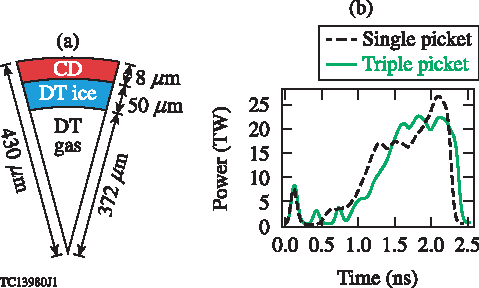
\includegraphics[width=80mm]{Fig1_Bose}
%\includegraphics{fig2_YOCvsIVP_dc}% Here is how to import EPS art
\caption{\label{fig:Exp_pulse_target} The pulse shapes and targets from the ``50-Gbar" implosions.\cite{Exp_Regan}}
\end{figure}
%
%
%
%
%%% %%%%%%                                                TABLE            %%%%%%%%%%%%%%%%
%\clearpage
%\begin{landscape}
\begin{table*}
\caption{\label{tab:Exp_1} This table lists the experimental observable and the corresponding 1-D estimate from simulations [in brackets] for the ensemble of cryogenic implosions on OMEGA which produced $\sim$50 Gbar pressure. In the column showing areal density ($\rho R$) both NTOF and MRS (second) measurements are listed.}
\begin{ruledtabular}
\begin{tabular}{c c c c c c c c}
%\hline

%& & & & & & &\\

Shot & $Y (\times 10^{13})$ & x-ray $R_{17\%}$ ($\mu$m) & $T_\text{i}$ (keV) & $\Delta T_\text{i}$ (keV) & $\rho R$ (mg/cm$^2$) & Burnwidth (ps) & $P$ (Gbar) \\


 & $\pm 5 \%$ & $\pm 0.5$ $\mu$m & $\pm 0.3$ keV &  & $\pm 31$, $\pm 19$ mg/cm$^2$ & $\pm 10$ ps & $\pm 7$ Gbar  \\  \hline
% & & & & & & &\\ \hline %\hhline{|=||=|=|=|=|=|=|=|} %\hhline{=|=|=}
% & & & & & & &\\
\\

78959 &   4.39  & 21.3  & 3.63 & 0.54 & 213, 203 & 71      & 52 \\ 
\vspace{2mm}
         &  [13.8] &[20.9]&  [3.6]&        &  [232]     & [54.1]& [109] \\
%         & & & & & & &\\ %\hline
%         & & & & & & &\\

78963 & 4.38 & 22.1 & 3.69   &0.88 & 204, 208  & 67     & 49 \\
\vspace{2mm}
         &[16.3]&[19.8]& [3.74]&       &[242]        &[51.1]&[126]  \\  
%         & & & & & & &\\ %\hline
%         & & & & & & &\\

78967 & 3.76  & 21.4  & 3.65& 0.85  & 179, 195 &	64  & 50 \\
\vspace{2mm}
         & [15.3]&[20.4]&[3.69]&        & [238]     &[51.1]& [120] \\ 
%         & & & & & & &\\ %\hline
%         & & & & & & &\\

78969 & 4.48  & 21.7   & 3.7   & 0.46 & 204, 197 & 59      & 55  \\
\vspace{2mm}
         &[14.1] & [21.4] &[3.66]&        &[216]       & [54.7]&[104] \\ 
%         & & & & & & &\\ %\hline
%         & & & & & & &\\

78971 & 3.77 &	22.1 & 3.69& 1.06 & 220, 208& 72    &	44 \\
\vspace{2mm}
         &[14.4] &[21.4]  &[3.64]&        & [222]     &[52.9]&[107]  \\ 
%         & & & & & & &\\ %\hline
%        & & & & & & &\\

77064  & 4.21  & 22.0   & 3.32&  0.42& 211, 191& 64     & 56  \\
\vspace{2mm}
          & [12.5]& [20.4] &[3.48]&      & [219]      & [57.4]&  [108] \\ 
%          & & & & & & &\\ %\hline
%          & & & & & & &\\

77066  & 4.11  & 21.9  & 3.18& 0.57& 221, 193& 70     & 56 \\
\vspace{2mm}
          & [16.1]&[21.4]&[3.66]&      &  [228]    &[52.9]&[112]  \\ 
%          & & & & & & &\\ %\hline
%          & & & & & & &\\

77068  & 5.3  & 22.  & 3.6  &  0.16& 211, 194  & 66   & 56 \\
\vspace{2mm}
          & [17.]&[22.]&[3.82]&        &[211]       &[56.7]& [97]  \\ 
%          & & & & & & &\\ %\hline
%         & & & & & & &\\

77070  & 4.02  & 20.3  &	3.4   & 0.23 & 220, 229  & 71     & 57  \\
%\vspace{2mm} 
           &[13.3]&[20.4] & [3.55]&        &[239]        &[52.6] &[114]\\
%           & & & & & & &\\ %\hline
% \hline
\end{tabular}
\end{ruledtabular}
\end{table*}
%\end{landscape}
%%%%%%%%%%%
%
%
%
%
%
%
%
%
%%% %%%%%%                                                FIGURE          %%%%%%%%%%%%%%%
\begin{figure}
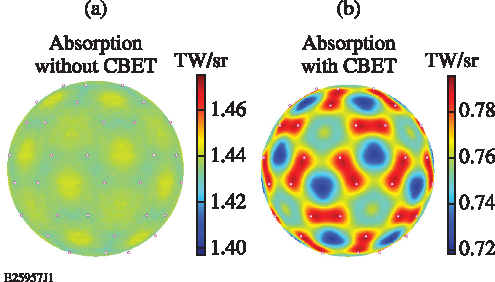
\includegraphics[width=80mm]{Fig2_Bose}
%\includegraphics{fig2_YOCvsIVP_dc}% Here is how to import EPS art
\caption{\label{fig:Exp_CBET}The laser power absorbed at the target surface is shown for calculations: (a) without considering cross-beam energy transfer (CBET) between the interacting laser beams, and (b) with CBET. [Reprint with permission, LLE Review, Vol. 150]}
\end{figure}
%
%


 It has been shown by Regan \textit{et al.}\cite{Exp_Regan} that direct-drive cryogenic implosions on OMEGA have achieved hot-spot pressures exceeding 50 Gbar---a performance that surpassed all previous implosions on OMEGA. The implosion performance was estimated based on the experimental observables: neutron yield, areal density, ion temperature, hot-spot volume, and neutron burnwidth. The ``50-Gbar" implosions used standardized pulse shapes (either a single-picket pulse or a triple-picket pulse) and standardized targets (shown in Fig. \ref{fig:Exp_pulse_target}). The 1-D performance is estimated from simulations using the hydrodynamic code \textit{LILAC}.\cite{Exp_LILAC1} It must be noted that the laser deposition models in \textit{LILAC} were optimized to reproduce in-flight observables like laser-energy deposition and shell trajectory.\cite{Exp_LILAC2, Exp_LILAC3} The estimated implosion adiabat for this design is $\alpha$ $\approx$3.5-to-4 (the adiabat $\alpha \propto P/P_\text{F}$ at the interface of the hot spot and shell at the time when the laser-driven shocks reach this interface, where $P$ represents the hydrodynamic pressure and $P_\text{F}$ is the Fermi pressure of a degenerate electron gas). It is considered to be a mid-adiabat implosion design, slightly above the indirect-drive ``high foot" design. The hot-spot pressure in 1-D is estimated to be $\sim$100 Gbar, close to the $\sim$120 Gbar required to demonstrate hydro-equivalent ignition (this is discussed in Refs. \onlinecite{Bose_RTIscaling_2015} and \onlinecite{Exp_Bose}). 

Table \ref{tab:Exp_1} lists the performance of several of these 50-Gbar implosions. The performance parameters are similar for all the shots. The neutron yields are $\sim$4$\times 10^{13}$, at a yield degradation level $Y/Y_\text{1D} \sim 0.3$. Where $Y_\text{1D}$ represents the post-shot 1-D simulation yield, calculated using \textit{LILAC}. The hot-spot radii for all the shots are $\sim$22 $\mu$m; they were estimated using time-resolved x-ray images\cite{Exp_Fred} (discussed in Sec. \ref{sec:Exp_gatedimage}). The ion temperatures ($T_\text{i}\sim 3.5$ keV) are comparable to the temperatures from 1-D simulations, to within 10$\%$ degradation level. The $T_\text{i}$'s were measured using three different detectors---the chemical vapor deposition (CVD) detector \cite{Exp_CVD} and the 12-m and 15-m neutron time-of-flight (nTOF) detectors \cite{Exp_NTOF1, Exp_NTOF2}---positioned along different implosion lines of sight. The variation in $T_\text{i}$ measurement $\Delta T$, which is the difference between the maximum and minimum measured temperatures, is greater than 10$\%$ for all of the shots. The measured areal densities are comparable to the 1-D estimates. The $\rho R$ is measured using the nTOF and magnetic recoil spectrometer (MRS) \cite{Exp_MRS} detectors. The measured burnwidths are slightly longer than the 1-D estimate. The burnwidths are measured using the neutron temporal diagnostic (NTD). \cite{Exp_NTD}
%
%
%

 For direct-drive implosions on OMEGA, it is anticipated that the core is degraded by a combination of low and intermediate modes. Although the origin of the asymmetries is uncertain, low modes can arise from several factors, including long-wavelength target defect, target positioning, laser beam balance and laser beam pointing.\cite{Exp_Hu, Exp_Goncharov, Exp_Igor} In addition, the superposition of all 60 laser beams on OMEGA can produce overlap intensity variations, which is expected to introduce intermediate-mode nonuniformities, similar to the $\ell=$6 or 10 modes in 2-D geometry. The cross-beam energy transfer (CBET) calculations by D. Edgell \textit{et. al},\cite{Exp_Edgell} shown in Fig. \ref{fig:Exp_CBET}, represent the variation in laser-energy absorption at the target surface. When CBET is included, the nonuniformity is higher by 10$\times$. These variations may be associated with the origin of mid-mode asymmetry in direct-drive implosions.
%
%
%
%
%
%
%
%
%
%
%\FloatBarrier
%%%%%%%%%%%%%%%%%%%%%%%%%%%%%%%%%%%%%%%%%%
%%%%%%%%%%%%%%%%%%%%%%%%%%%%%%%%%%%%%%%%%%
%%				SECTION2: Synthetic reconstruction technique
%%%%%%%%%%%%%%%%%%%%%%%%%%%%%%%%%%%%%%%%%%
%%%%%%%%%%%%%%%%%%%%%%%%%%%%%%%%%%%%%%%%%%
\section{The Reconstruction Technique and its Application}
\label{sec:Exp_technique}
%
%
%%% %%%%%%                                                FIGURE          %%%%%%%%%%%%%%%
\begin{figure}
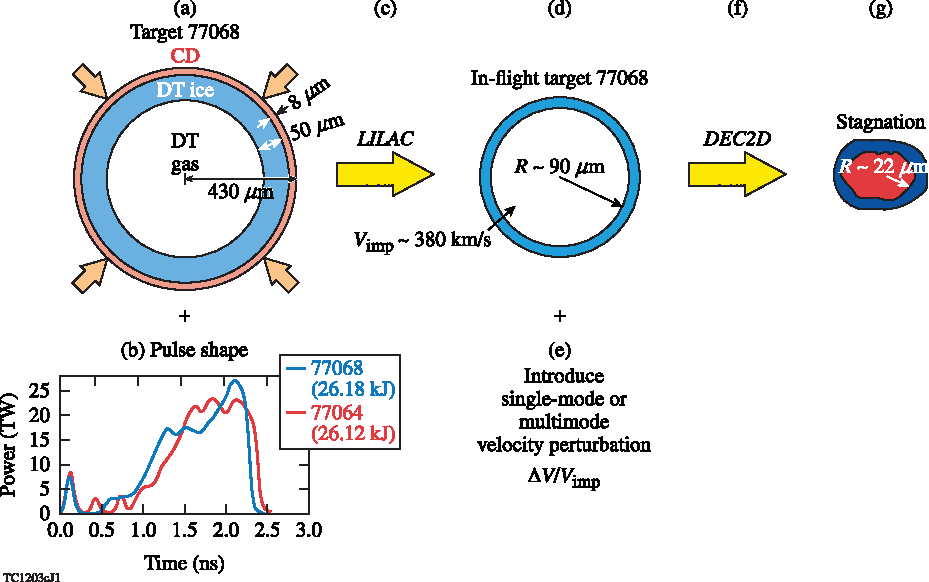
\includegraphics[width=85mm]{Fig3_Bose}
%\includegraphics{fig2_YOCvsIVP_dc}% Here is how to import EPS art
\caption{\label{fig:Exp_technique} The procedure involved in the reconstruction technique. The (a) target and (b) pulse shape are used as initial conditions for the 1-D hydrodynamic code \textit{LILAC}, which is used to (c) simulate the acceleration phase of implosions. The hydrodynamic profiles from the (d) in-flight target simulation are transferred to \textit{DEC2D}; single- or multimode velocity perturbations are (e) introduced at the inner surface of the shell. (f) The deceleration phase of the implosion is simulated in 2-D; (g) the stagnation parameters are extracted from these simulations.}
\end{figure}
%
%
%
%
%
%%% %%%%%%                                                FIGURE          %%%%%%%%%%%%%%%
\begin{figure}
\includegraphics{Fig4_Bose}
%\includegraphics{fig2_YOCvsIVP_dc}% Here is how to import EPS art
\caption{\label{fig:Exp_spectrum} This plot shows the initial velocity perturbation spectrum $\Delta V/V_{\text{imp}} \% (\ell)$ that was used to synthetically reconstruct the shot 77068.}
\end{figure}
%
%
%
%
%
%
%
%
%%% %%%%%%                                                FIGURE          %%%%%%%%%%%%%%%
\begin{figure}
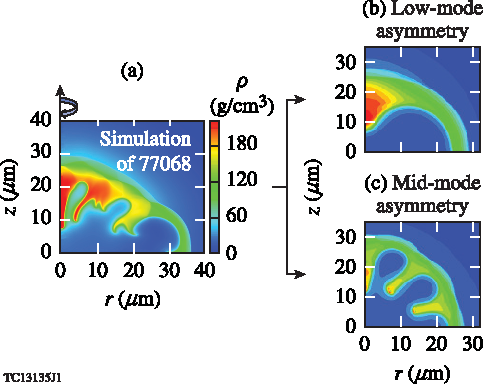
\includegraphics[width=80mm]{Fig5_Bose}
%\includegraphics{fig2_YOCvsIVP_dc}% Here is how to import EPS art
\caption{\label{fig:Exp_LowMid} This figure illustrates that combination of low and mid modes were used to reconstruct the core conditions of the shot 77068. The density profiles at time of peak neutron production are shown for (a) the reproduced shot 77068, (b) the low-mode $\ell=2$ component and (c) an equivalent mid-mode $\ell=10^*$ component.}
\end{figure}
%
%

Unlike the conventional approach that involves full simulations of the implosions including nonuniformities from numerous sources, our technique focuses only on the final phase of an implosion. The final phase consists of the deceleration phase followed by stagnation and disassembly, which are critical in the production of fusion reaction neutrons detected by the nuclear diagnostics. They also produce bremsstrahlung emission detected by the x-ray imaging diagnostics. Performance degradation results from a combination of nonuniformities: they are amplified by the RTI during the acceleration phase and can feed through to the inner surface, where they are further amplified during the deceleration phase by the RTI. 
%
%
%
%
%

 The radiation--hydrodynamic code \textit{DEC2D} is used to simulate the deceleration phase of implosions. The details of the code have been discussed in Ref. \onlinecite{Bose_RTIscaling_2015}. As outlined in Fig. \ref{fig:Exp_technique}, the acceleration phase was simulated using \textit{LILAC}.\cite{Exp_LILAC1} It includes the laser drive with models for CBET\cite{Exp_LILAC2} and nonlocal thermal transport.\cite{ Exp_LILAC3} The hydrodynamic profiles at the end of the laser pulse were used as initial conditions for the deceleration-phase simulations in 2-D. Initial perturbations for the deceleration-phase RTI were introduced at the interface of the shell and the hot spot through angular variation of the velocity field.
%
%

Here we consider three categories of degradation: low-mode asymmetry, mid-mode asymmetry, and 1-D degradation. The low-mode trends are represented using a mode 2 ($\ell=2$) and phase reversed mode 2 (denoted using ``$\ell=2$ ph. rev."); the RTI spike axis coincides with the simulation axis of symmetry for the former and they are orthogonal for the latter. The mid-mode trends are represented using a $\ell=10^*$ and a multimode spectrum referred to as ``mid modes". The $\ell=10^*$ consists of a central mode $\ell=10$ along with sideband modes $\ell=8$ and 12 at 20$\%$ of central mode amplitude. The ``mid modes" consist of a spectrum of modes given by $4 \leq \ell \leq 20$ at the same amplitude and a $1/\ell^2$ roll-off spectrum for higher modes $20 \leq \ell \leq 100$. In simulations, the implosion performance was degraded by increasing the peak amplitude but the shape of the spectrum was preserved. The 1-D degradation is incorporated as a degradation in the implosion velocity of the shell, i.e., degradation in the initial condition of the deceleration-phase simulations; this has been denoted using ``1-D Vimp."    
%
%

  The pulse shape and target from OMEGA shot 77068 (used in this analysis) are shown in Fig. \ref{fig:Exp_technique}. The analysis technique is very robust and can be applied to any implosion and any scale. The choice of shot 77068 was motivated by the fact that this was the best shot in terms of performance metric $\chi_{\text{no-}\alpha}$\cite{Exp_Bose, Betti-alphaheat} and other experimental observables. The target was driven with 26.18 kJ of laser energy to an implosion velocity of 380 km/s. The experimental observables, the 1-D simulation parameters, and the reconstructed observables for this shot are shown in Table \ref{tab:Exp_2}. Notice that the experimental observables were reproduced using the 2-D simulations. The velocity perturbation used for this is shown in Fig. \ref{fig:Exp_spectrum}; it consists of a combination of low- and mid-mode asymmetries. Figure \ref{fig:Exp_LowMid} shows the shape of the hot spot and shell at time of peak neutron production (i.e., bang time $t_\text{b}$). The final shape resembles a combination of a low-mode $\ell=2$, and a dominant mid-mode $\ell=10$. We emphasize that the exact mode numbers degrading the experimental performance cannot be inferred from this analysis technique, and other combinations of modes could also lead to the same reconstructed observables. However, the overall balance between the degradation by low modes and the degradation by mid modes on all of the observables must be preserved. To illustrate this, we also show trends from a different low mode: the $\ell=2$ asymmetry with a reversed phase. Although this mode has a different structure, the resulting trends are the same; for example, see trends in pressure and volume degradation in Figs. \ref{fig:Exp_pressure} and \ref{fig:Exp_volume}. Similarly, the mid modes (of the spectrum in Fig. \ref{fig:Exp_spectrum}) resembles the mode $\ell=10^*$.        

 The following sections show the analysis of the 50-Gbar implosion results using this technique. The effect of low and mid modes on each of the implosion observables is discussed.
%
%
%
%
%
%%%%%%%%%%%%%%
%%%%%%%%%%%%%%
%%%%%%%%%%%%%%
%%Table1
\begin{table*}
%\begin{center}
\caption{\label{tab:Exp_2}Comparison of measurements with 1-D simulations (using \textit{LILAC} and \textit{DEC2D}) and 2-D simulations (using \textit{DEC2D}).}
\begin{ruledtabular}
%\scalebox{0.85}{
\begin{tabular}{c c c c c c}
%\hline
 Observables & Experiment & 1-D sim. & Reconstructed & Mid modes & $\ell=2$ \\
  & shot 77068 &   & shot 77068 & Component (1) & Component (2) \\

\hline
%\hhline{|=||=|=|=|=|=|}
\\

Yield& $5.3\times 10^{13}(\pm 5\%)$ & $1.7\times 10^{14}$ & $5.3\times 10^{13}$ & $7.9\times 10^{13}$ & $9.8\times 10^{13}$ \\
$P^*$ (Gbar)& 56($\pm$7) & 97 & 57 & 77 & 73\\
$T_{\text{ion}}$ (keV)& 3.6($\pm 0.3$) & 3.82 & 3.7 & 3.78 & 3.71 \\
$R_{\text{hs}}$ ($\mu$m)& 22($\pm1$) & 22 & 22 & 20.9 & 23.4 \\
$\tau$ (ps)& 66($\pm 10$) & 61 & 54 & 55 & 56 \\
$\rho R$ (g/cm$^2$)& 0.194($\pm0.018$) & 0.211 & 0.194 & 0.222 & 0.203 \\
%\hline
\end{tabular}%}
%\end{center}
\end{ruledtabular}
\end{table*}
%%%%%%%%%%%%%%
%%%%%%%%%%%%%%
%
%
%
%
%
%
%\FloatBarrier
%%%%%%%%%%%%%%%%%%%%%%%%%%%%%%%%%%%%%%%%%%
%%%%%%%%%%%%%%%%%%%%%%%%%%%%%%%%%%%%%%%%%%
%%				SECTION3: Pressure
%%%%%%%%%%%%%%%%%%%%%%%%%%%%%%%%%%%%%%%%%%
%%%%%%%%%%%%%%%%%%%%%%%%%%%%%%%%%%%%%%%%%%
%%%%%%%%%%%%%%%%%%%%%%%%%%%%%%%%%%%%%%%%%%
\subsection{Inferred Hot-Spot Pressure}
\label{sec:Exp_pressure}
%
%
%
%
%%% %%%%%%                                                FIGURE          %%%%%%%%%%%%%%%
\begin{figure}
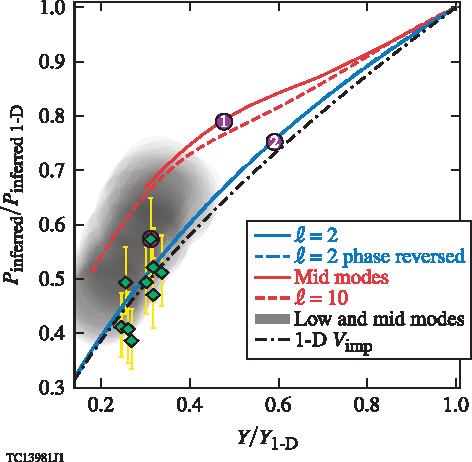
\includegraphics[width=80mm]{Fig6_Bose}
%\includegraphics{fig2_YOCvsIVP_dc}% Here is how to import EPS art
\caption{\label{fig:Exp_pressure} Figure showing the degradation in inferred hot-spot pressure $P_\text{Inferred}$, normalized with 1-D pressure ($P_\text{Inferred-1D}$), versus degradation in yield ($Y/Y_\text{1D}$). The `50 Gbar' shots, in Table \ref{tab:Exp_1}, are shown in green. The reconstructed shot 77068 is shown in magenta (overlapping the experimentally inferred pressure for 77068), with points (1) and (2) representing the degradation caused by the mid-mode and low-mode components separately. The gray shaded region represents an ensemble of simulations using different amplitude combination of $\ell=2$ and mid-modes, it is observed that these reproduce the experiments.}
\end{figure}
%
%
The hot-spot pressure is not directly measurable but it is inferred from other observables using \cite{Exp_SC}
%
%
%
%-----------
\begin{eqnarray}
\label{eqn:Exp_pressure}
\frac{P_\text{inferred}}{P_\text{inferred 1D}} =  \hspace{55mm} \nonumber
\\
\sqrt{ \left( \frac{Y}{Y_\text{1D}} \right)  \left( \frac{V}{V_\text{1D}} \right)^{-1}   \left[ \frac{\left( \left< \sigma v  \right>/T_\text{i}^2 \right)}{\left( \left< \sigma v  \right>/T_\text{i}^2 \right)_\text{1D}} \right]^{-1}  \left( \frac{\tau}{\tau_\text{1D}} \right)^{-1}  } \hspace{5mm},
\end{eqnarray}
%-----------
%
%
where $Y$ is the implosion yield obtained from experiments or simulations and is normalized with the 1-D yield ($Y_\text{1D}$) from simulations. The $V/V_\text{1D}$ is the normalized volume of the hot spot, calculated from the x-ray images of experiments or simulations. The fusion reactivity is a function of temperature only,\cite{Exp_Bosch} $\left< \sigma v \right>/T_\text{i}^2 \sim T_\text{i}^\sigma$, with $\sigma \approx 1$-to-$2$ for the temperature range of interest to ICF. The neutron burnwidth $\tau$ is the full width at half maximum of the neutron rate and can be obtained from experiments or simulations. The degradation trends for each of these observables will be shown in the following sections. 

 The degradation in pressure corresponding to a given degradation in yield is shown in Fig. \ref{fig:Exp_pressure}. The degradation in inferred pressure is an outcome of the degradation in all of the measurable parameters shown in Eq. (\ref{eqn:Exp_pressure}). For any yield degradation level, the low modes (in blue) result in a greater degradation of the hot-spot pressure as compared to mid modes (in red). The `$\ell=2$' and `$\ell=2$ ph. rev.' produce similar pressure degradation curves; also the `$\ell=10^*$' and `mid modes' produce similar curves. This is because for `mid modes' the hot-spot volume is smaller as a result of cooling by penetration of the RTI spikes, but for low modes the volume is larger (see Sec. \ref{sec:Exp_gatedimage}). The gray-shaded region represents an ensemble of simulations using different amplitude combinations of `$\ell=2$' and `mid modes'; with the $\ell=2$ amplitude varying between $4 \%$ and $7\%$ of $V_\text{imp}$ and the 'mid-modes' amplitude varying between $2\%$ and $4\%$ of $V_\text{imp}$. The combination of initial velocity perturbation shown in Fig. \ref{fig:Exp_spectrum} could be used to reproduce the experimental pressure for shot 77068. The dashed black line shows the 1-D pressure scaling with implosion velocity; it follows $P_\text{inferred} \sim V_\text{imp}^{3.72}$. The corresponding yield scaling with implosion velocity follows $Y \sim V_\text{imp}^{6.26}$. The implosion velocity degradation is a simplistic method to model the degradation in implosion convergence; it is useful only for comparison of trends. In experiments, degradation in implosion convergence can be caused by the following: very short scale nonuniformities arising from laser imprinting or reduced laser-to-capsule drive with respect to simulation, and preheating caused by super-thermal electrons (which decrease the implosion convergence by increasing the implosion adiabat $\alpha$). 

 Notice that the pressure degradation curve for the `1D Vimp' coincides with the low-mode curves but is different from the `mid modes'. This can be explained based on Ref. \onlinecite{Bose_physics_2017}. It is so because, firstly, the isobaric hot-spot approximation is not valid for implosions with mid-mode asymmetries, and, secondly, the inferred pressure for mid modes is the average pressure of the x-ray--producing region of the hot spot. The x-ray--producing volume, however larger than the burn volume (i.e., neutron-producing volume), is still smaller than the total hot-spot volume including the bubbles (i.e., $V_{\left< \text{hs} \right>}$ of Ref. \onlinecite{Bose_physics_2017}). As a result, the inferred pressure for implosions with mid-mode asymmetry is higher than the average hot-spot pressure.

%
%\FloatBarrier
%%%%%%%%%%%%%%%%%%%%%%%%%%%%%%%%%%%%%%%%%%
%%%%%%%%%%%%%%%%%%%%%%%%%%%%%%%%%%%%%%%%%%
%%				SECTION3: SIZE
%%%%%%%%%%%%%%%%%%%%%%%%%%%%%%%%%%%%%%%%%%
%%%%%%%%%%%%%%%%%%%%%%%%%%%%%%%%%%%%%%%%%%
\subsection{Estimation of the Hot-Spot Size: Using Time-Gated Self-Emission Images}
\label{sec:Exp_gatedimage}
%
%
 Time-resolved images of the core x-ray self-emission, as shown in Fig. \ref{fig:Exp_kbframed}, have been used to estimate the hot-spot volume. Here $R_{17}$ is the radius at 17$\%$ of peak intensity and $V_\text{x-ray}/V_\text{x-ray-1D} = (R_{17}/R_{17-\text{1D}})^3$.
%
%
%%% %%%%%%                                                FIGURE          %%%%%%%%%%%%%%%
\begin{figure}
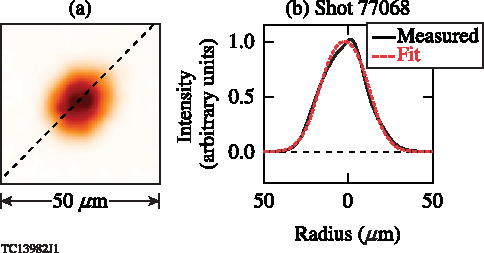
\includegraphics[width=80mm]{Fig7_Bose}
%\includegraphics{fig2_YOCvsIVP_dc}% Here is how to import EPS art
\caption{\label{fig:Exp_kbframed} (a) An x-ray image of the hot-spot at stagnation for the shot 77068, obtained using a time resolved Kirkpatrick-Baez (KB) framed camera with a 4--8 keV photon energy range and a $\sim$ 6 $\mu$m spatial resolution.\cite{Exp_Fred} The measured and fitted x-ray profiles along the dashed line are shown in (b).}
\end{figure}
%
%
%
%
%
%
%
%%% %%%%%%                                                FIGURE          %%%%%%%%%%%%%%%
\begin{figure}
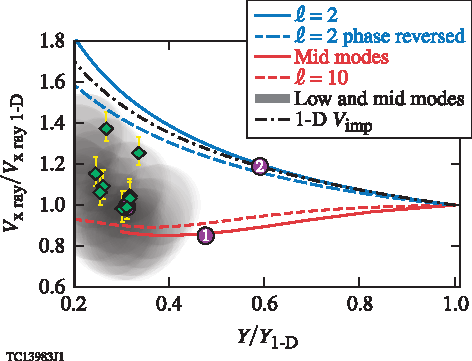
\includegraphics[width=80mm]{Fig8_Bose}
%\includegraphics{fig2_YOCvsIVP_dc}% Here is how to import EPS art
\caption{\label{fig:Exp_volume} Plot showing the volume of the hot spot, obtained from time resolved x-ray images and normalized with the 1-D volume ($V_\text{x-ray}/V_\text{x-ray-1D}$), versus the yield degradation $Y/Y_\text{1D}$. The `50 Gbar' shots, in Table \ref{tab:Exp_1}, are shown in green. The reconstructed shot 77068 is shown in magenta (overlapping the x-ray volume for the shot 77068), with points (1) and (2) representing the degradation caused by the mid-mode and low-mode components separately. The gray shaded region represents an ensemble of simulations using different amplitude combination of $\ell=2$ and mid-modes, it is observed that these reproduce the experiments.}
\end{figure}
%
%
%

The effect of asymmetries on the hot-spot volume is shown in Fig. \ref{fig:Exp_volume}. It is shown that with increasing mode amplitude the x-ray volume increases for low modes and decreases for `mid modes'. By cooling the plasma within the RTI bubbles, mid mode asymmetries cause a reduction in the x-ray emitting volume. The gray shaded region (representing the ensemble of simulations) shows that the volume estimated using a combination of low and mid modes is in agreement with the measured volume for the `50 Gbar' shots. Illustrating that the experiments can be reconstructed using such combinations of low and mid-modes. The effect of an implosion velocity degradation (i.e., `1D Vimp') on the x-ray volume has been shown using the black dashed line, it follows the scaling $V_\text{x-ray} \sim V_\text{imp}^{-2.14}$. Notice that this curve coincides with the low mode curve, but is different from the mid mode asymmetry curves; it is so for the same reasons as previously explained.

 Time resolved x-ray images (i.e., with 10 ps gate width) were produced from the simulations using the atomic physics code \textit{SPECT3D}. These images were normalized with the maximum intensity for each image and fit with the following function,
%
%-----------
\begin{equation}
\label{eqn:Exp_supergaussian}
f(x,y) = e^{-\left[ (x/a)^2 + (y/b)^2 \right]^{\eta/2}}.
\end{equation}
%-----------
%
 The $R_{17}$ was obtained from the fit using, $R_{17} = \sqrt{a\times b} [-\text{log}(0.17)]^{1/\eta}$. The index $\eta$ represents the index of the Super-Gaussian fit, with $\eta=2$ representing a Gaussian function. The disassembly phase of implosions is different for low-modes and mid-modes, as discussed in Ref. [\onlinecite{Bose_physics_2017}]. During the disassembly (i.e., for $t > t_\text{b}$) the $R_{17}$ decreases with time for mid modes, whereas it increases for low modes. And the index $\eta$ decreases for mid-modes and increases for low modes. These are shown in Fig. \ref{fig:Exp_volumeVstime}. Since detection of mid-modes in experiments is challenging due to the limited spatial resolution of the detectors', the above time evolution trends in the x-ray images could motivate future experiments.
%
%
%
%%% %%%%%%                                                FIGURE          %%%%%%%%%%%%%%%
\begin{figure}
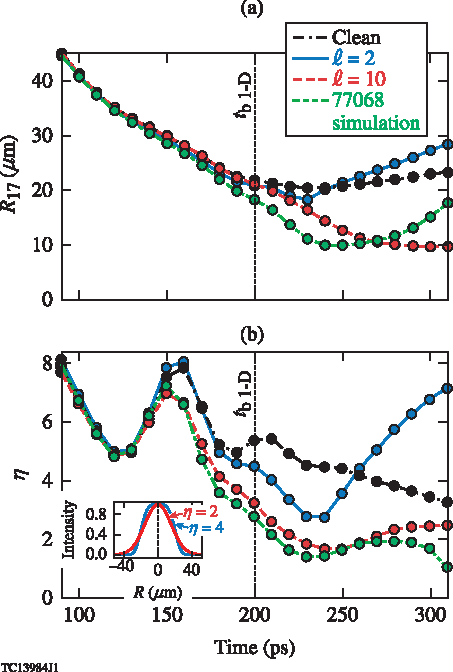
\includegraphics[width=80mm]{Fig9_Bose}
%\includegraphics{fig2_YOCvsIVP_dc}% Here is how to import EPS art
\caption{\label{fig:Exp_volumeVstime} (a) Plot showing the time evolution of the x-ray $R_{17}$ obtained from simulations. This is shown for the symmetric case (black line), low mode $\ell=2$ case with $Y/Y_\text{1D}=0.6$ (blue line), mid mode $\ell=10$ case with $Y/Y_\text{1D}=0.6$ (red line), and the reproduced case with $Y/Y_\text{1D}\approx 0.3$ (green line) for simulations of shot 77068. (b) Plot showing the time evolution of the Super-Gaussian $\eta$ for the x-ray emission profile (see Eq. \ref{eqn:Exp_supergaussian}) for the above mentioned implosion simulations.}
\end{figure}
%
%
%
%
%\FloatBarrier
%%%%%%%%%%%%%%%%%%%%%%%%%%%%%%%%%%%%%%%%%%
%%%%%%%%%%%%%%%%%%%%%%%%%%%%%%%%%%%%%%%%%%
%%				SECTION2: Shape 
%%%%%%%%%%%%%%%%%%%%%%%%%%%%%%%%%%%%%%%%%%
%%%%%%%%%%%%%%%%%%%%%%%%%%%%%%%%%%%%%%%%%%
\subsection{Shape Analysis of Time-Integrated Self Emission Images}
\label{sec:Exp_intimage}
%
%
%
%%% %%%%%%                                                FIGURE          %%%%%%%%%%%%%%%
\begin{figure*}
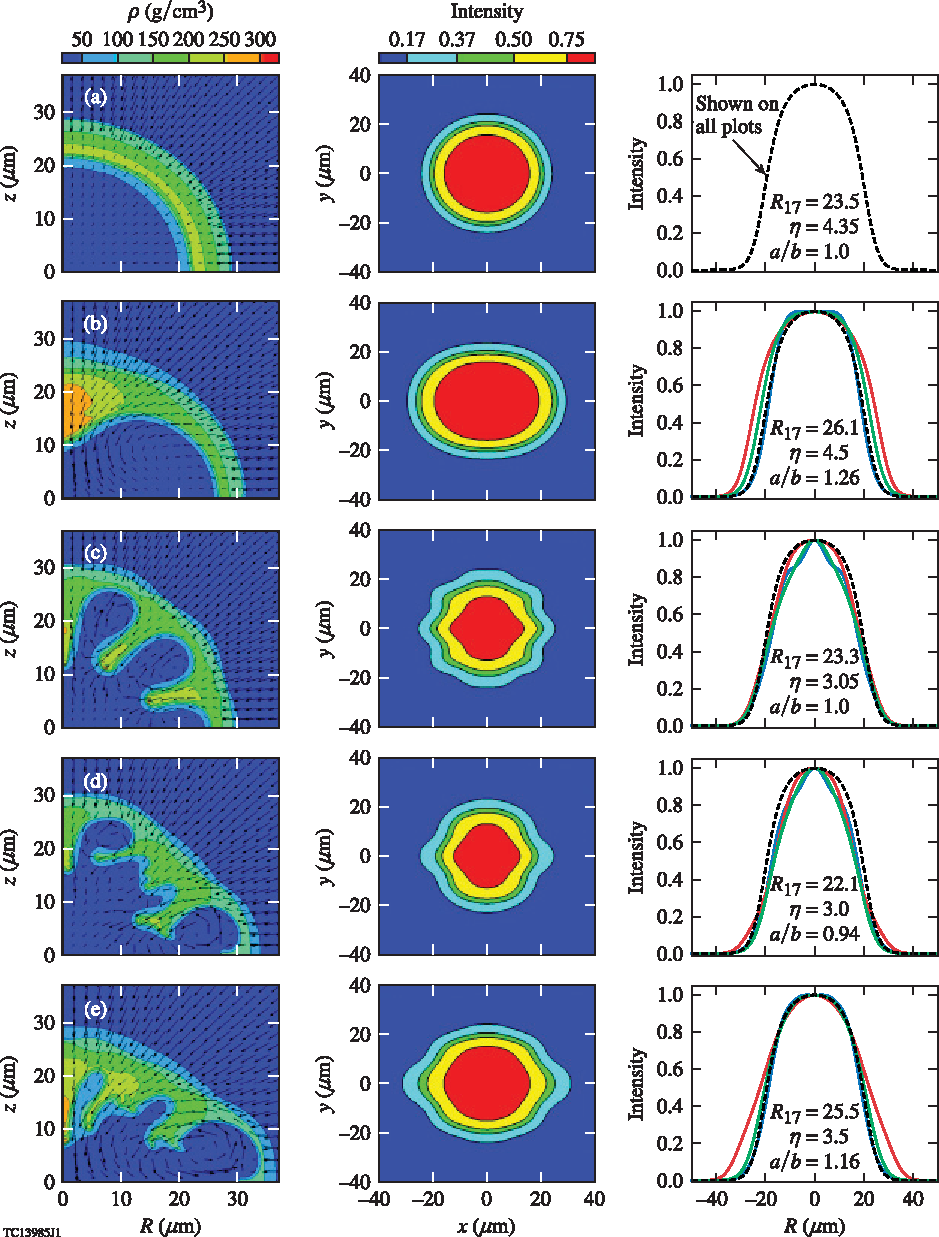
\includegraphics{Fig10_Bose}
%\includegraphics{fig2_YOCvsIVP_dc}% Here is how to import EPS art
\caption{\label{fig:Exp_shape1} \footnotesize{Contour plots of the density profile and plasma flow pattern at bang time (first column), time integrated synthetic x-ray emission images (second column), and image lineouts (third column) are shown. The black dashed line represents the lineout of the symmetric image, it is shown on all plots. The lineouts along the three different axis are labeled with different colors (red, blue and green). The 2-D Super-Gaussian fit parameters have been included. The images for (a) symmetric implosion, (b) $\ell=2$ at $Y/Y_\text{1D}=0.6$, (c) $\ell=10$ at $Y/Y_\text{1D}=0.6$, (d) `mid modes' with 2$\%$ $\Delta V$ at $Y/Y_\text{1D}=0.47$, and (e) reconstructed shot 77068 are shown.}}
\end{figure*}
%
%
%
%
%
%
%%% %%%%%%                                                TABLE            %%%%%%%%%%%%%%%%
%\clearpage
%\begin{landscape}
\begin{table}
%\begin{center}
\caption{\label{tab:Exp_3} Table showing the properties for the time integrated GMXI x-ray images from experiments.}
\begin{ruledtabular}

\begin{tabular}{c c c c c}

Shot & $R_{17}$ ($\mu$m) & $\eta$ & $a/b$ & filter  \\


 & $\pm 0.5$ $\mu$m & $\pm$ 0.2 & $\pm$ 0.01  & 6.5 mil Be +\\ 

\hline
%\hhline{|=||=|=|=|=|} %\hhline{=|=|=}

\\
78959 &   25.6  & 2.7  & 1.16 &  3 mil Al  \\   %\hline

78963 &  28.1 & 2.3 & 1.17  & 3 mil Al \\  %\hline

78967 & 26.7  & 2.3  & 1.16 & 3 mil Al \\ %\hline

78969 & 27.4  & 2.6   & 1.16  &  3 mil Al \\ %\hline

78971 & 27.1  & 1.9 &  1.20 & 3 mil Al \\ %\hline

77064  & 27.7  & 2.6   & 1.11 &   2 mil Al \\ %\hline

77066  & 26.8  & 2.6  & 1.1 & 2 mil Al \\ %\hline

77068  & 26.7 &  2.94  & 1.16  &  2 mil Al \\ %\hline

77070  & 25.9  & 2.56  &	1.13   & 2 mil Al \\ 
%\hline

\end{tabular}
%\end{center}
\end{ruledtabular}
\end{table}
%\end{landscape}
%%%%%%%%%%%
%
%
%
%
%
%
%
%%% %%%%%%                                                FIGURE          %%%%%%%%%%%%%%%
\begin{figure}
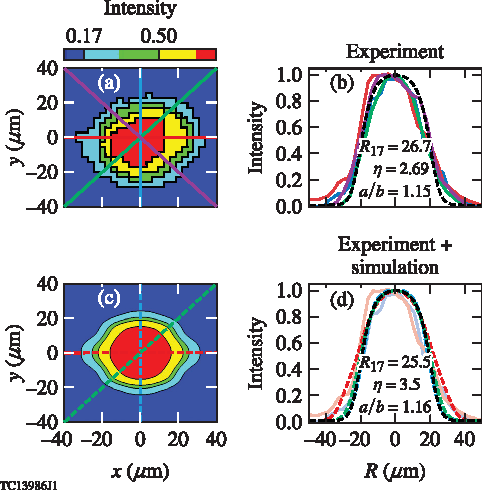
\includegraphics{Fig11_Bose}
%\includegraphics{fig2_YOCvsIVP_dc}% Here is how to import EPS art
\caption{\label{fig:Exp_shape2} Figure showing a comparison between time integrated x-ray images for the shot 77068 obtained from (a-i) experiments and (b-i) from the reconstructed simulation. The lineouts along the different axis are labeled with different colors (red, blue, green and magenta), the lineouts for the experimental image are represented using solid lines (in a-ii and b-ii) and the simulations are represented using dashed lines (in b-ii). The lineout for the symmetric case is shown with black dashed line (in a-ii and b-ii). The Super-Gaussian fit parameters for both experiment (in a-ii) and simulation (in b-ii) are listed.}
\end{figure}
%

In this section we discuss how asymmetries influence the time integrated x-ray images. Since the photon statistics (i.e., determined by the number of incident photons) is insufficient for the 10--15 ps time gated images, we do not use these images to infer the shape of the hot-spot; instead the time integrated images obtained using the gated monochromatic x-ray imaging (GMXI) module \cite{Exp_GMXI} are used. In Fig. \ref{fig:Exp_shape1} the first column shows the density profile and flow pattern at bang time. The corresponding synthetic self-emission images along with line-outs across different axis are shown in the second and third columns. The cross sections are taken through the center of the image, they are marked on the contour plot with the same color as on the intensity plot. The x-ray images are reconstructed with the same filter and point spread function (PSF) as the experimental shot 77068, i.e., filtered with 6.5 mil of Be and 2 mil of Al, which transmits x-rays in the 4-8 keV range, and a 7.5 $\mu$m PSF. The images were fit using the function shown in Eq. \ref{eqn:Exp_supergaussian}. The $R_{17}$ of the time integrated images, the ellipticity parameter ($a/b$), and the Super-Gaussian exponent $\eta$ are calculated from the fit. It is found that low modes cause an increase in the $a/b$ and $R_{17}$, with the index-$\eta$ comparable or larger than the 1-D case. Instead mid-modes cause a reduction in the index $\eta$. This is because the mid-modes exhibit several low temperature bubbles surrounding the hot center, producing a more gradual intensity variation with radius. 
%
%
%
%

 Table \ref{tab:Exp_3} shows the properties of the time integrated x-ray images for the `50 Gbar' shots. It is observed that for all of the shots the time integrated $R_{17}$ is larger than the time resolved images by $\sim$ 3--4 $\mu$m, which is in consistent agreement with our analysis. The $\eta < \eta_\text{1D}$ indicates the presence of mid-modes and the $a/b>1$ indicates the presence of low-modes in the implosions.


 Figure \ref{fig:Exp_shape2} shows the time integrated image for the shot 77068 and the reconstructed image for the same. The agreement in shape, and other parameters ($R_{17}$,$a/b$ and $\eta$) reassures the presence of systematic mid-modes along with low-modes in the `50 Gbar' implosions. In summary, low modes increase the ellipticity parameter ($a/b$) and radius ($R_{17}$) from the time integrated x-ray images, and mid-modes produce a lower Super-Gaussian index $\eta$. A combination of low- and mid-mode asymmetry can be used to reproduce the experimental images. 
%
%
%
%
%\FloatBarrier
%%%%%%%%%%%%%%%%%%%%%%%%%%%%%%%%%%%%%%%%%%
%%%%%%%%%%%%%%%%%%%%%%%%%%%%%%%%%%%%%%%%%%
%%				SECTION4: Ion Temperature
%%%%%%%%%%%%%%%%%%%%%%%%%%%%%%%%%%%%%%%%%%
%%%%%%%%%%%%%%%%%%%%%%%%%%%%%%%%%%%%%%%%%%
\subsection{Neutron Averaged Ion Temperature}
\label{sec:Exp_temperature}
%
%
%
%%% %%%%%%                                                FIGURE          %%%%%%%%%%%%%%%
\begin{figure}
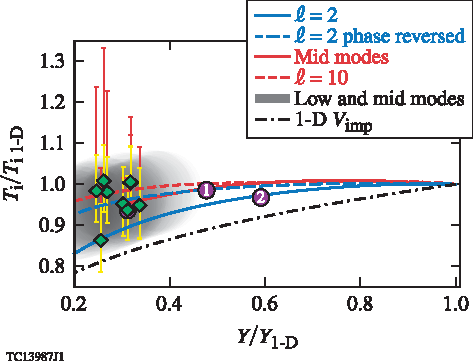
\includegraphics[width=80mm]{Fig12_Bose}
%\includegraphics{fig2_YOCvsIVP_dc}% Here is how to import EPS art
\caption{\label{fig:Exp_temp} Plot showing degradation in neutron averaged ion temperature ($T_\text{i}/T_\text{i-1D}$) versus the degradation in yield ($Y/Y_\text{1D}$). The points in green represent the minimum ion temperature measured for the `50 Gbar' shots; the red bar associated with each data point represents the maximum ion temperature measurement. The reconstructed shot 77068 is shown in magenta (overlapping with data), the points (1) and (2) represent degradation caused by the mid-mode and low-mode components separately. The gray shaded region represents an ensemble of simulations using different amplitude combination of $\ell=2$ and mid-modes, it is observed that these reproduce the experiments.}
\end{figure}
%
%
%
%
%
%
%%% %%%%%%                                                FIGURE          %%%%%%%%%%%%%%%
\begin{figure}
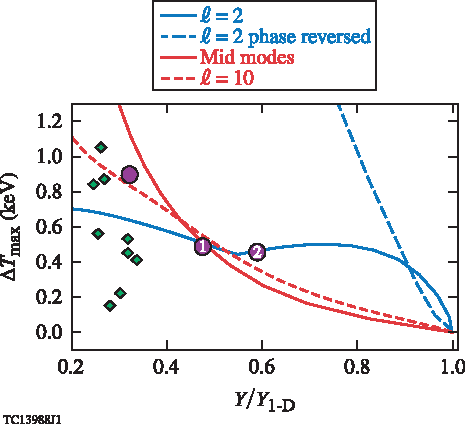
\includegraphics[width=80mm]{Fig13_Bose}
%\includegraphics{fig2_YOCvsIVP_dc}% Here is how to import EPS art
\caption{\label{fig:Exp_tempVar} 
Plot showing the maximum variation in ion temperature measurements ($\Delta T_\text{max}$) versus degradation in yield ($Y/Y_{1D}$). For the `50 Gbar' experiments, shown in green, the $\Delta T_\text{max}$ is given by $\Delta T_\text{max} = T_\text{i-max}- T_\text{i-min}$ across measurements along different lines of sight. The simulations show maximum variation in ion temperature given by $\Delta T_\text{max} = \text{Max}(T_\text{spike-axis},T_\text{bubble-axis})- T_\text{i}$, where $T_\text{n-avg}$ is the neutron-averaged ion temperature and $T_\text{spike-axis}$, $T_\text{bubble-axis}$ are apparent temperature along spike and bubble axis respectively.
}
\end{figure}
%
%


Figure \ref{fig:Exp_temp} shows the degradation in ion temperature ($T_\text{i}/T_\text{i-1D}$) with degradation in yield $(Y/Y_\text{1D})$. It is observed that asymmetries cause a small degradation in $T_\text{i}/T_\text{i-1D}$, within $10-15 \%$ of the 1-D value, for all yield degradation level above $Y/Y_\text{1D}>0.2$. This is because the temperature of the region of the hot-spot that produces fusion neutrons, i.e., the hot region, is only marginally affected by asymmetries (see Ref. [\onlinecite{Bose_physics_2017}]). Marked in gray are the results from simulations with a combination of low and mid mode asymmetries. The points in green, representing the `50 Gbar' experiments, fall within the gray region. In 1-D the temperature scaling with implosion velocity follows $T_\text{i} \sim V_\text{imp}^{0.91}$, this is estimated from the black dashed line. It is observed that at the same yield degradation ($Y/Y_\text{1D}$) the temperature degradation is greater for `1D Vimp' than asymmetries.

The variation in ion temperature measurements between detectors is shown using the red bars, the length of the bar is proportional to $\Delta T_\text{max}=T_\text{i-Max} -T_\text{i-Min}$ between measurements. Bulk flows in the neutron producing region of the hot spot, marked with arrows in Fig. \ref{fig:Exp_shape1} (first column), can affect the temperature measurements. It can result in a higher measured temperature depending on the line of sight of the detector. The variation in neutron averaged ion temperature versus yield degradation level is shown in Fig. \ref{fig:Exp_tempVar}. For the simulations the apparent temperature (i.e., including flow effects) were calculated, using the Murphy \textit{et al.}\cite{murphy_the_2014} formulation. The maximum variation possible is estimated using [$\Delta T_\text{max} = \text{Max}(T_\text{spike-axis}, T_\text{bubble-axis})- T_\text{i}$], where $T_\text{spike-axis}$ (or $T_\text{bubble-axis}$) is the apparent temperature measured by a detector sitting on the spike-axis (or bubble-axis) and $T_\text{i}$ is the neutron averaged ion temperature calculated not including the flow effects. We find that the $\Delta T_\text{max}$ from experiments and the calculated $\Delta T_\text{max}$ are comparable for implosions with $\ell=2$ and mid-modes. The phase reversed mode (`$\ell=2$ ph. rev.') produces higher variation in apparent temperature than others. 

In summary, our technique using a combination of low and mid modes can be used to consistently reproduce the neutron averaged temperature measurements and estimate the variation in temperature for the `50 Gbar' experiments. 
%
%
%
%
%
%\FloatBarrier
%%%%%%%%%%%%%%%%%%%%%%%%%%%%%%%%%%%%%%%%%%
%%%%%%%%%%%%%%%%%%%%%%%%%%%%%%%%%%%%%%%%%%
%%				SECTION5: RhoR estimation
%%%%%%%%%%%%%%%%%%%%%%%%%%%%%%%%%%%%%%%%%%
%%%%%%%%%%%%%%%%%%%%%%%%%%%%%%%%%%%%%%%%%%
\subsection{Implosion Areal Density}
\label{sec:Exp_rhoR}
%
%
%
%%% %%%%%%                                                FIGURE          %%%%%%%%%%%%%%%
\begin{figure}
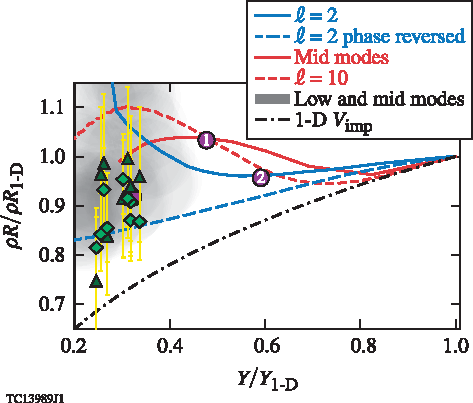
\includegraphics[width=80mm]{Fig14_Bose}
%\includegraphics{fig2_YOCvsIVP_dc}% Here is how to import EPS art
\caption{\label{fig:Exp_rhoR} Plot showing the degradation in areal density $\rho R$ versus degradation in yield, the $\rho R$ and yield are normalized with the 1-D estimated values. The NTOF (triangles) and MRS (diamonds) $\rho R$ measurements for the `50 Gbar' shots are shown in green. The reconstructed shot 77068 is shown in magenta (overlapping with data), with points (1) and (2) representing degradation caused by the mid-mode and low-mode components separately. The gray shaded region represents an ensemble of simulations using different amplitude combination of $\ell=2$ and mid-modes, it is observed that these reproduce the experiments.}
\end{figure}
%
%
%
%
 The effect of asymmetries on the areal density $\rho R$ is discussed in this section, the $\rho R$ obtained from experiments and simulations are shown in Fig. \ref{fig:Exp_rhoR}. It is observed that the measured $\rho R$s are comparable to the 1-D estimated values, although, the yields are heavily degraded $Y/Y_\text{1D} \sim 0.3$. In the simulations the neutron averaged integral $\rho \text{d}r$ was calculated along radial lines.

 The $\rho R$ scaling with implosion velocity is shown with the black dashed line (`1D Vimp'); %, it follows $\rho R \sim V_\text{imp}^{1.68}$. 
notice that the $\rho R$ for implosions with asymmetries is always higher than this curve. The $\rho R$ is a parameter dependent on the implosion convergence; for symmetric implosions the yield decreases with decreasing convergence. Instead for distorted implosions, the convergence of the spikes can be high but this does not increase the yield (see Ref. [\onlinecite{Bose_physics_2017}]). At high yield degradation ($Y/Y_\text{1D} < 0.4$), the $\rho R$ for $\ell =2$ and $\ell=10^*$ (with single mode RTI) is greater than the estimated $\rho R_\text{1D}$. This is because the RTI spikes approach the implosion center producing a compressed plasma with a higher $\rho R$. For the `mid modes' case this effect is reduced. For the` $\ell=2$ ph. rev.' case, the spike lies on the implosion waist; the massive spike converges less and the $\rho R$ increase is modest. 

  A combination of low and mid modes (shown by the gray region) could be used to reconstruct the $\rho R$ for the `50 Gbar' shots (shown in green). The measurements along with consideration of the asymmetry trends suggests that a fraction of the measured $\rho R$ could be contribution from the cold spikes and bubbles surrounding the burn volume, therefore, they do not contribute in fusion yield production.
%
%
%
%
%\FloatBarrier
%
%%%%%%%%%%%%%%%%%%%%%%%%%%%%%%%%%%%%%%%%%%
%%%%%%%%%%%%%%%%%%%%%%%%%%%%%%%%%%%%%%%%%%
%%				SECTION6: Tau
%%%%%%%%%%%%%%%%%%%%%%%%%%%%%%%%%%%%%%%%%%
%%%%%%%%%%%%%%%%%%%%%%%%%%%%%%%%%%%%%%%%%%
\subsection{Burnwidth and Bang Time}
\label{sec:Exp_bwandbt}
%
%
%
%
%
%%% %%%%%%                                                FIGURE          %%%%%%%%%%%%%%%
\begin{figure}
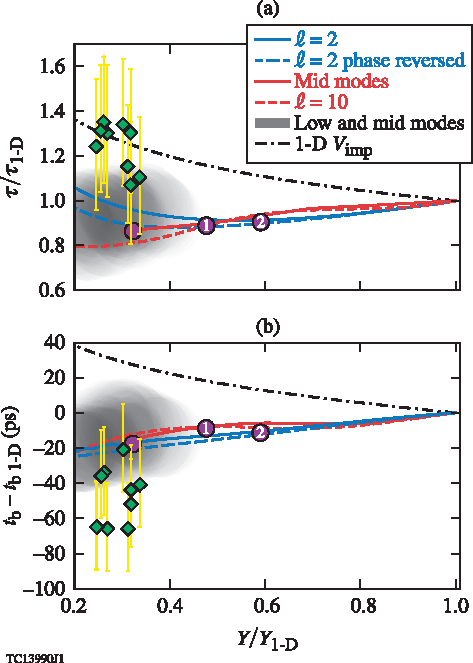
\includegraphics[width=80mm]{Fig15_Bose}
%\includegraphics{fig2_YOCvsIVP_dc}% Here is how to import EPS art
\caption{\label{fig:Exp_BW_BT}\small{Plots showing (a) burnwidth $( \tau/\tau_\text{1D} )$ and (b) shift in bang time with respect to the 1-D simulations (i.e., $t_\text{b}-t_\text{b-1D}$), versus degradation in yield ($Y/Y_\text{1D}$). The points in green represent the experimental results from the `50 Gbar' implosions (Tab. \ref{tab:Exp_1}). The reconstructed shot 77068 is shown in magenta, the points (1) and (2) represent degradation caused by the mid-mode and low-mode components separately. The gray shaded region represents an ensemble of simulations using different amplitude combination of $\ell=2$ and mid-modes.}}
\end{figure}
%

%
%
%
%
%%% %%%%%%                                                FIGURE          %%%%%%%%%%%%%%%
%\begin{figure}[h!]
%\begin{center}
%\includegraphics[width=120mm]{asymmetry_exp/BangTime}
%%\includegraphics{fig2_YOCvsIVP_dc}% Here is how to import EPS art
%\caption{\label{fig:Exp_bangtime} Plot showing the variation in bang time with respect to the 1-D simulations (i.e., $t_\text{b}-t_\text{b-1D}$) versus degradation in yield $Y/Y_\text{1D}$.  The points in green represent the `50 Gbar' shots. The reconstructed shot 77068 is shown in magenta, with points (1) and (2) representing degradation with the mid-mode and low-mode components separately. The gray shaded region represents an ensemble of simulations using different amplitude combination of $\ell=2$ and mid-modes, it is observed that these reproduce the experiments.
%}
%\end{center}
%\end{figure}
%
%

Figure \ref{fig:Exp_BW_BT}(a) shows a plot of burnwidth degradation ($\tau/\tau_\text{1D}$) with yield degradation ($Y/Y_\text{1D}$). It is observed that the burnwidths from NTD measurements are longer than the 1-D calculated value ($\tau/\tau_\text{1D} > 1$); however, the estimated error in the NTD burnwidths is considerable. The scaling of burnwidth with implosion velocity is represented using the `1D Vimp' curve, it follows $\tau \sim V_\text{imp}^{-1.2}$.

 In simulations with asymmetries, the burnwidth shows a modest reduction with degradation in yield. However, for very large low-mode asymmetries (i.e., $Y/Y_\text{1D}<0.4$) the burnwidth increases with decreasing yield; this is described in Ref. [\onlinecite{Bose_physics_2017}]. Combination of low and mid modes (shown with gray) produce burnwidths that are comparable to the 1-D burnwidth (to within $\pm 30\%$), but on an average they are shorter than the burnwidths for the `50 Gbar' implosions.

%
%
%
%
%
 The Fig. \ref{fig:Exp_BW_BT}(b) shows shift in bang time compared to the 1-D estimated values $(t_\text{b}-t_\text{b-1D})$ with degradation in yield ($Y/Y_\text{1D}$). The bang time from experiments (measured using the NTD) are shifted forward in time; however, the estimated error in the NTD bang times are considerable. Notice that unlike burnwidths, this is in agreement with the asymmetry trends which also shift the bang time forward; but it is opposite to what an implosion velocity degradation would do, i.e., `1-D Vimp' shifts the bang time later, $(t_\text{b}-t_\text{b-1D}) > 0$. 

 We propose three possible explanations for the discrepancy between burnwidth and bang time. One possibility is the inaccuracy of the measurements. The NTD measurements for burnwidth and bang time have large error bars, and probably are influenced by systematic effects that are not being considered. It is possible that the actual burnwidths are 10-15 ps shorter, and the actual bang time times are 10-15 ps later than what is measured. The 10-15 ps in both burnwidth and bang-time are within the measurement error. This would mean that both are consistent with the trends arising from asymmetries.

 The second possibility is that there is a low mode asymmetry (not considered here) that is causing an increase in burnwidth, and simultaneously shifts the bang time earlier. We speculate that it could be the outcome of a $\ell=1$ mode. This is based on the observation that for very large $\ell=2$ asymmetry (i.e., $Y/Y_\text{1D}< 0.4$), the $\tau$ increases with a decrease in yield. The implosion dynamics along the orthogonal directions (i.e., along the pole and the waist) are sufficiently mismatched in time, causing a prolonged but inefficient compression, i.e., an increase in $\tau$ although the yield is low. We speculate that this effect on the burnwidth may be enhanced for a $\ell=1$ asymmetry, which involves larger bulk flow. This could not be verified because the \textit{DEC2D} simulation domain is currently restricted to a $90^o$ wedge (see Ref. \onlinecite{Bose_RTIscaling_2015}) instead of the full 360$^o$ required for a $\ell=1$ simulation.

The most likely explanation is that there is a 1-D degradation in implosion convergence in addition to a low mode (like the $\ell =2$) and a mid mode (like the $\ell =10$). This would mean that there is a systematic difference in the laser drive that is not accounted for by the laser plasma coupling models in the \textit{LILAC} simulations. Therefore the burnwidths are indeed longer, as measured by the NTD and predicted by the `1D Vimp' scaling curves. However, the bang time which depends on the history of the acceleration-phase is not correctly captured by the simplistic deceleration-phase (`1D Vimp') scaling.  

%
%
%
%
%
%%%%%%%%%%%%%%%%%%%%%%%%%%%%%%%%%%%%%%%%%%
%%%%%%%%%%%%%%%%%%%%%%%%%%%%%%%%%%%%%%%%%%
%%				SECTION6: Conclusion
%%%%%%%%%%%%%%%%%%%%%%%%%%%%%%%%%%%%%%%%%%
%%%%%%%%%%%%%%%%%%%%%%%%%%%%%%%%%%%%%%%%%%
\section{Conclusions and Future Application}
\label{sec:Exp_summary}
%
%
%%% %%%%%%                                                FIGURE          %%%%%%%%%%%%%%%
%%%%%%%%%%%%%%
\begin{figure}
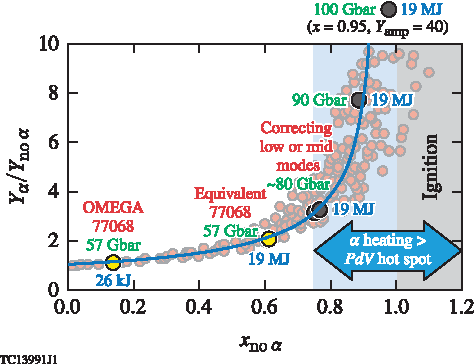
\includegraphics[width=85mm]{Fig16_Bose}
\caption{\label{Fig3} Plot of yield amplification versus $\chi_{\text{no-}\alpha}$,\cite{Betti-alphaheat} with 1-D and 2-D simulation results are shown in red, and the curve $Y_\alpha/Y_{\text{no-}\alpha} = (1-\chi_{\text{no-}\alpha}/0.96)^{-0.75}$ is shown in blue. The Lawson ignition condition $\chi_{\text{no-}\alpha}\geq 1$ and the burning plasma regime $Q_\alpha \geq 1$ are shown by the gray and blue regions respectively. The OMEGA shot 77068 and its equivalent implosion extrapolated to a 1.9 MJ driver are shown in yellow, they exhibit inferred core pressures of 57 Gbar. Correcting either the low-mode or mid-mode component of this implosion can produce $\approx 80$ Gbar pressure (see Table \ref{tab:Exp_2}), with its performance approaching the burning plasma regime; the 1-D design has a hot-spot pressure of $\approx$100 Gbar.}
\end{figure}
%%%%%%%%%%%%%%
%
 In this paper a technique to investigate the implosion performance degradation mechanisms was discussed, based on trends in the experimental measurable. This was applied to an ensemble of DT cryogenic implosions on OMEGA that achieved hot-spot pressures exceeding 50 Gbar.\cite{Exp_Regan} It was shown that a combination of low- and mid-mode asymmetries could be used to reconstruct the implosion core.\cite{Exp_Bose} In addition to the presence of low modes, which cause a degradation of the stagnation pressure, it was shown that mid-mode asymmetries have a significant impact on the implosion performance. While imaging of mid-mode asymmetries in implosions is challenging, this technique can be used to infer the effect of mid-modes on the observables. It was shown that mid modes decrease the hot-spot size (i.e., time-resolved x-ray $R_{17}$), and lead to center peaked time-integrated x-ray images (i.e., a smaller Super-Gaussian exponent $\eta$ compared to a symmetric implosion). This occurs because the region of mid-mode bubbles surrounding the hot-center introduces a gradual variation in the x-ray intensity. A consistent explanation for the ion-temperature, areal density, volume, and pressure measurements for the `50 Gbar' shots was described. The possible reasons behind the modest discrepancies between burnwidth and bang time was discussed based on the measurements and the predicted degradation trends. 

 A combination of low- and mid-modes was used to reconstruct all the experimental observables pertaining to the core. Mitigation of low- and mid-mode asymmetries would both result in an increase of the fusion yield, through an increase of the hot-spot pressure (from 56 Gbar to 80 Gbar) for low modes, and an increase in the burn volume for mid-modes. Figure \ref{Fig3} shows that an improvement in implosion core symmetry resulting from either correction of the low-mode or mid-modes, included in the reconstruction of shot 77068 (and other `50 Gbar' shots \cite{Exp_Regan}), can produce a burning plasma (i.e., $Q_\alpha \geq 1 $  \cite{Betti-alphaheat}) when extrapolated to 1.9 MJ.\cite{Exp_Bose} 

 In future this analysis technique will be applied to different 1-D implosion designs. This would enhance the understanding and possibly lead to identification of the degradation sources for the OMEGA direct-drive implosions. 
%
%%%%%%%%%%%%%%%%%%%%%%%%%%%
%%%%%%%%%%%%%%%%%%%%%%%%%%%
%
%
%%%%%%%%%%%%%%%%%%%%%%%%%%%%%%%%%%%%%%%%%%
%%%%%%%%%%%%%%%%%%%%%%%%%%%%%%%%%%%%%%%%%%
%%				SECTION2: Acknowledgments
%%%%%%%%%%%%%%%%%%%%%%%%%%%%%%%%%%%%%%%%%%
%%%%%%%%%%%%%%%%%%%%%%%%%%%%%%%%%%%%%%%%%%
%%%%%%%%%%%%%%%%%%%%%%%%%%%%%%%%%%%%%%%%%%
\section{Acknowledgments}
\label{acknowledgments}
%
%
 This research has been supported by the U.S. Department of Energy under Cooperative Agreements DE-FC02-04ER54789 (Office of Fusion Energy Sciences) and DE-NA0001944 (National Nuclear Security Administration), and by the NYSERDA. This report was prepared as an account of work sponsored by an agency of the U.S. Government. Neither the U.S. Government nor any agency thereof, nor any of their employees, makes any warranty, express or implied, or assumes any legal liability or responsibility for the accuracy, completeness, or usefulness of any information, apparatus, product, or process disclosed, or represents that its use would not infringe privately owned rights. Reference herein to any specific commercial product, process, or service by trade name, trademark, manufacturer, or otherwise does not necessarily constitute or imply its endorsement, recommendation, or favoring by the U.S. Government or any agency thereof. The views and opinions of authors expressed herein do not necessarily state or reflect those of the U.S. Government or any agency thereof.
%
%
%
%%%%%%%%%%%%%%%%%%%%%%%%
%\cleardoublepage
\begin{thebibliography}{5}
%
\bibitem{nuckolls_laser_1972}J. Nuckolls, L. Wood, A. Thiessen, and G. Zimmerman, Nature 239, 139 (1972).
%
\bibitem{betti_inertial-confinement_2016}R. Betti and O. A. Hurricane, Nat. Phys. 12, 435 (2016).
%
\bibitem{bodner_direct-drive_1998}S. E. Bodner, D. G. Colombant, J. H. Gardner, R. H. Lehmberg, S. P. Obenschain, L. Phillips, A. J. Schmitt, J. D. Sethian, R. L. McCrory, W. Seka, C. P. Verdon, J. P. Knauer, B. B. Afeyan, and H. T. Powell, Phys. Plasmas 5, 1901 (1998).
%
\bibitem{lindl_development_1995}J. D. Lindl, Phys. Plasmas 2, 3933 (1995).
%
\bibitem{betti_deceleration_2002}R. Betti, K. Anderson, V. N. Goncharov, R. L. McCrory, D. D. Meyerhofer, S. Skupsky, and R. P. J. Town, Phys. Plasmas 9, 2277 (2002).
%
\bibitem{Exp_Regan}S. P. Regan, V. N. Goncharov, I. V. Igumenshchev, T. C. Sangster, R. Betti, A. Bose, T. R. Boehly, M. J. Bonino, E. M. Campbell, D. Cao, T. J. B. Collins, R. S. Craxton, A. K. Davis, J. A. Delettrez, D. H. Edgell, R. Epstein, C. J. Forrest, J. A. Frenje, D. H. Froula, M. Gatu Johnson, V. Yu. Glebov, D. R. Harding, M. Hohenberger, S. X. Hu, D. Jacobs-Perkins, R. T. Janezic, M. Karasik, R. L. Keck, J. H. Kelly, T. J. Kessler, J. P. Knauer, T. Z. Kosc, S. J. Loucks, J. A. Marozas, F. J. Marshall, R. L. McCrory, P. W. McKenty, D. D. Meyerhofer, D. T. Michel, J. F. Myatt, S. P. Obenschain, R. D. Petrasso, R. B. Radha, B. Rice, M. Rosenberg, A. J. Schmitt, M. J. Schmitt, W. Seka, W. T. Shmayda, M. J. Shoup III, A. Shvydky, S. Skupsky, S. Solodov, C. Stoeckl, W. Theobald, J. Ulreich, M. D. Wittman, K. M. Woo, B. Yaakobi, and J. D. Zuegel, Phys. Rev. Lett. 117, 025001 (2016).

\bibitem{Bose_physics_2017}A. Bose, R. Betti, D. Shvarts, and K. M. Woo, Phys. Plasmas 24, 102704 (2017).

\bibitem{Exp_LILAC1}J. Delettrez, R. Epstein, M. C. Richardson, P. A. Jaanimagi, and B. L. Henke, Phys. Rev. A 36, 3926 (1987).

\bibitem{Exp_LILAC2}I. V. Igumenshchev, W. Seka, D. H. Edgell, D. T. Michel, D. H. Froula, V. N. Goncharov, R. S. Craxton, L. Divol, R. Epstein, R. Follett, J. H. Kelly, T. Z. Kosc, A. V. Maximov, R. L. McCrory, D. D. Meyerhofer, P. Michel, J. F. Myatt, T. C. Sangster, A. Shvydky, S. Skupsky, and C. Stoeckl, Phys. Plasmas 19, 056314 (2012).

\bibitem{Exp_LILAC3}V. N. Goncharov, T. C. Sangster, P. B. Radha, R. Betti, T. R. Boehly, T. J. B. Collins, R. S. Craxton, J. A. Delettrez, R. Epstein, V. Yu. Glebov, S. X. Hu, I. V. Igumenshchev, J. P. Knauer, S. J. Loucks, J. A. Marozas, F. J. Marshall, R. L. McCrory, P. W. McKenty, D. D. Meyerhofer, S. P. Regan, W. Seka, S. Skupsky, V. A. Smalyuk, J. M. Soures, C. Stoeckl, D. Shvarts, J. A. Frenje, R. D. Petrasso, C. K. Li, F. Seguin, W. Manheimer, and D. G. Colombant, Phys. Plasmas 15, 056310 (2008).

\bibitem{Bose_RTIscaling_2015}A. Bose, K. M. Woo, R. Nora, and R. Betti, Phys. Plasmas 22, 072702 (2015).

\bibitem{Exp_Bose}A. Bose, K. M. Woo, R. Betti, E. M. Campbell, D. Mangino, A. R. Christopherson, R. L. McCrory, R. Nora, S. P. Regan, V. N. Goncharov, T. C. Sangster, C. J. Forrest, J. Frenje, M. Gatu Johnson, V. Yu. Glebov, J. P. Knauer, F. J. Marshall, C. Stoeckl, and W. Theobald, Phys. Rev. E 94, 011201(R) (2016).

\bibitem{Exp_Fred}F. J. Marshall, R. E. Bahr, V. N. Goncharov, V. Yu. Glebov, B. Peng, S. P. Regan, T. C. Sangster, and C. Stoeckl, LLE Review, Volume 150 (2017).

\bibitem{Exp_CVD}G. J. Schmid et al., Rev. Sci. Instrum. 74, 1828 (2003).

\bibitem{Exp_NTOF1}V.Y. Glebov, D.D. Meyerhofer, C. Stoeckl, and J.D. Zuegel, Rev. Sci. Instrum. 72, 824 (2001).

\bibitem{Exp_NTOF2}V. Yu. Glebov, C. J. Forrest, K. L. Marshall, M. Romanofsky, T. C. Sangster, M. J. Shoup III, and C. Stoeckl, Rev. Sc. Instrum. 85, 11E102 (2014).

\bibitem{Exp_MRS}J.A. Frenje, D.T. Casey, C.K. Li, J.R. Rygg, F.H. Séguin, R.D. Petrasso, V.Yu Glebov, D.D. Meyerhofer, T.C. Sangster, S. Hatchett \textit{et al.}, Rev. Sci. Instrum. \textbf{79}, 10E502 (2008).

\bibitem{Exp_NTD}C. Stoeckl, R. Boni, F. Ehrne, C. J. Forrest, V. Yu. Glebov \textit{et al.}, Rev. Sci. Instrum. 87, 053501 (2016)


\bibitem{Exp_Hu}S. X. Hu, P. B. Radha, J. A. Marozas, R. Betti, T. J. B. Collins, R. S. Craxton, J. A. Delettrez, D. H. Edgell, R. Epstein, V. N. Goncharov, I. V. Igumenshchev, F. J. Marshall, R. L. McCrory, D. D. Meyerhofer, S. P. Regan, T. C. Sangster, S. Skupsky, V. A. Smalyuk, Y. Elbaz, and D. Shvarts, Phys. Plasmas 16, 112706 (2009).


\bibitem{Exp_Goncharov}V. N. Goncharov, T. C. Sangster, R. Betti, T. R. Boehly, M. J. Bonino, T. J. B. Collins, R. S. Craxton, J. A. Delettrez, D. H. Edgell, R. Epstein, R. K. Follet, C. J. Forrest, D. H. Froula, V. Yu. Glebov, D. R. Harding, R. J. Henchen, S. X. Hu, I. V. Igumenshchev, R. Janezic, J. H. Kelly, T. J. Kessler, T. Z. Kosc, S. J. Loucks, J. A. Marozas, F. J. Marshall, A. V. Maximov, R. L. McCrory, P. W. McKenty, D. D. Meyerhofer, D. T. Michel, J. F. Myatt, R. Nora, P. B. Radha, S. P. Regan, W. Seka, W. T. Shmayda, R. W. Short, A. Shvydky, S. Skupsky, C. Stoeckl, B. Yaakobi, J. A. Frenje, M. Gatu-Johnson, R. D. Petrasso, and D. T. Casey, Phys. Plasmas 21, 056315 (2014).

\bibitem{Exp_Igor}I. V. Igumenshchev, D. T. Michel, R. C. Shah, E. M. Campbell, R. Epstein \textit{et al.}, Phys. Plasmas 24, 056307 (2017)

\bibitem{Exp_Edgell}D. H. Edgell, R. K. Follett, I. V. Igumenshchev, J. F. Myatt, J. G. Shaw \textit{et al.}, Phys. Plasmas 24, 062706 (2017); ``Mitigation of Cross-Beam Energy Transfer in Symmetric Implosions on OMEGA Using Wavelength Detuning", LLE Review, Volume 150 (2017).

\bibitem{Betti-alphaheat}R. Betti, A.R. Christopherson, B.K. Spears, R. Nora, A. Bose, J. Howard, K.M. Woo, M.J. Edwards, and J. Sanz, Phys. Rev. Lett. 114, 255003 (2015).

\bibitem{Exp_SC}C. Cerjan, P. T. Springer, and S. M. Sepke, Phys. Plasmas 20, 056319 (2013).

\bibitem{Exp_Bosch}H. S. Bosch and G. M. Hale, Nucl. Fusion 32, 611 (1992); 33, 1919(E) (1993).

\bibitem{Exp_GMXI}F. J. Marshall and J. A. Oertel, Rev. Sci. Instrum. \textbf{68}, 735 (1997).


\end{thebibliography}
%
%
%
\end{document}
%
% ****** End of file aiptemplate.tex ******